\documentclass[a4paper,oneside,14pt]{memoir}
\usepackage{aubecse}

\settitle{Second Order Predictive Commoning in LLVM compiler Infrastructure}
\setnauthors{3}
\setauthorone{N. MD FAIZAAN}{2013103512}
\setauthortwo{MUTHURAJ M T}{2013103515}
\setauthorthree{ASWIN P}{2013103535}
\setguide{Dr. Arul Siromoney}{Professor}
\bachelors % Bachelors of Engineering
\university{Anna University}
\setgraddate{May 2015}

\usepackage{listings}
\usepackage{color}
\usepackage{float}
\usepackage{algorithm}
\usepackage{algorithmic}
\definecolor{dkgreen}{rgb}{0,0,0}
\definecolor{gray}{rgb}{0,0,0}
\definecolor{mauve}{rgb}{0,0,0}

\lstset{frame=tb,
  language=Java,
  aboveskip=3mm,
  belowskip=3mm,
  showstringspaces=false,
  columns=flexible,
  basicstyle={\small\ttfamily},
  numbers=none,
  numberstyle=\tiny\color{gray},
  keywordstyle=\color{gray},
  commentstyle=\color{dkgreen},
  stringstyle=\color{mauve},
  breaklines=true,
  breakatwhitespace=true,
  tabsize=3
}

\begin{document}
\frontmatter
\thetitlepage
\aucertificate
\auacknowledge
\auabstract
\auabstracttamil

%
\tableofcontents*
\listoffigures
\listoftables
\listofacronyms{CDMA}

\mainmatter
\pagestyle{au}
%\OnehalfSpacing
\auSpacing  % 0.8 cm using \baselineskip

%
% Chapter 1

\chapter{INTRODUCTION} % Write in your own chapter title All Chapter headings in CAPS
\section{Objective} % All Section headings in Title Case
Low Level Virtual Machine(LLVM) by Latner \textsl{et. al} \cite{Lattner:2004:LCF:977395.977673} is a compiler framework designed to support transparent, lifelong program analysis and transformation for arbitrary programs, by providing high-level information to compiler transformations at compile-time, link-time, run-time, and in idle time between runs. LLVM defines a common, low-level code representation in Static Single Assignment (SSA) form, and uses a universal Intermediate Representation (IR) for representing code at a level slightly above the assembly code. LLVM has matured into a full fledged compilation ecosystem with Clang being an excellent multi-stage optimizing compiler that can be a drop in replacement for GCC. We aim to implement Predictive commoning, a kind of loop optimization, in the LLVM compiler infrastructure.

\section{Problem Statement}
In loops, array accesses are often sequential in nature. This leads to use of same value from one iteration to next. Currently, the compiler loads the  value again which is redundant. We try to optimize this step by removing the load and inserting a register swap. 

\section{Need for the system}
LLVM applies loop optimizations to the generated IR, as a part of the optimization passes run by default. They include Loop Deletion, Loop extract, Loop reduce, Loop rotate, Loop Unroll, Loop unswitch and Loop simplify. However, LLVM does not apply optimization for loops in any predictive manner. While its GCC counterpart applies the predictive commoning, LLVM applies no such optimization. We implement second order predictive commoning to the LLVM infrastructure as a loadable module which can be invoked using a special flag.

\section{Challenges}

The main challenge of this project lies in program correctness. Any modification to the code must not result in incorrect code. For example, hoisting an array access must not result in undefined behavior. To overcome these, we employ Run Time Type Identification(RTTI) checks and make sure we don't optimize code incorrectly.

\section{Overview of thesis}
Chapter 2 discusses existing work in this area, including approaches to optimizations similar to what we are attempting. Chapter 3 explains the overall architecture and the design of various modules. Chapter 4 gives the implementation details of the project and discusses the results of optimization with emphasis on comparison between the execution times of various scenarios. Chapter 5 concludes the thesis and states the various extensions that can be made to the project. Appendix A explains the basic set up needed to work with LLVM. % Introduction
% Chapter 2
\chapter{RELATED WORK} % Chapter Title in ALL CAPSacs
Loops are a common target of various compiler optimization techniques. LLVM itself by default supports up to 10 optimizations targeted at loops. However there still is a lot left to be done especially in the area of reducing data accesses within the loops.

Oh \textsl{et al.} \cite{oh2013practical} discuss exploiting predictable patterns of values across loop iterations, as existing specializers cannot fully capitalize on this opportunity. To address this limitation, they have presented Invariant-induced Pattern based Loop Specialization (IPLS), the first fully-automatic specialization technique. Using dynamic information-flow tracking, IPLS profiles the values of instructions that depend solely on invariants and recognizes repeating patterns across multiple iterations of hot loops. IPLS then specializes these loops, using those patterns to predict values across a large window of loop iterations. This enables aggressive optimization of the loop.

Another style of optimization is with regard to invariants in a loop. LLVM includes ‘loop invariant code motion’ but Sharma \textsl{et al.} \cite{sharma2013data} focuses on algebraic invariants found through a data-driven approach. The task of generating loop invariants lies at the heart of any program verification technique. A wide variety of techniques have been developed for generating linear invariants, including methods based on abstract interpretation and constraint solving among others. Recently, researchers have also applied these techniques to the generation of non-linear loop invariants. These techniques discover algebraic invariants.

	
Current parallelization techniques handle instruction level parallelization well in a satisfactory manner, but when it comes to parallelization across of loop iterations, it’s not exploited well. Aiken and Nicolau \cite{aiken1988optimal} present a new technique bridging the gap between fine- and coarse-grain loop parallelization, allowing the exploitation of parallelism inside and across loop iterations. Furthermore, they show that, given a loop and a set of dependencies between its statements, the execution schedule obtained by out transformation is time optimal: no transformation of the loop based on the given data-dependencies can yield a shorter running time for that loop.


Wolf and Lam \cite{wolf1991data} talk about improving the data locality. It is achieved by loop transformation algorithm which is based on two concepts: a mathematical formulation of reuse and locality, and a loop transformation theory that unifies the various transforms as uni-modular matrix transformations. The algorithm is successful in optimizing programs such as matrix multiplication, successive over-relaxation, LU decomposition without pivoting, and Givens QR factorization. Performance evaluation indicates that locality optimization is especially crucial for scaling up the performance of parallel code.


Amato \textsl{et al.} \cite{amato2012discovering} propose a new technique combining dynamic and static analysis of programs to find linear invariants. They use a statistical tool, called simple component analysis, to analyze partial execution traces of a given program. They get a new coordinate system in the vector space of program variables, which is used to specialize numerical abstract domains.

Most conventional compilers fail to allocate array elements to registers because standard data-flow analysis treats arrays like scalars, making it impossible to analyze the definitions and uses of individual array elements. This deficiency is particularly troublesome for floating-point registers, which are most often used as temporary repositories for subscripted variables. In Callahan \textsl{et. al} \cite{callahan1990improving}, the authors present a source-to-source transformation, called scalar replacement, that finds opportunities for reuse of subscripted variables and replaces the references involved by references to temporary scalar variables. The objective is to increase the likelihood that these elements will be assigned to registers by the coloring-based register allocators found in most compilers. In addition, they present transformations to improve the overall effectiveness of scalar replacement and show how these transformations can be applied in a variety of loop nest types.

Wolf and Lam \cite{wolf1991loop} propose a new approach to transformations for general loop nests. In this approach, they unify all combinations of loop interchange, skewing and reversal as unimodular transformations. The use of matrices to model transformations has previously been applied only to those loop nests whose dependences can be summarized by distance vectors. Their technique is applicable to general loop nests where the dependences include both distances and directions.

Predictive commoning is a rather new approach applied in optimising loops by combining and modifying two earlier known methods namely, ’Common Subexpression Elimination’ and ’Loop-Invariant Code Motion’. It involves predicting whether array accesses will be reused in subsequent iterations and then tries to optimize those accesses by promoting them to registers. % Literature Survey
% Chapter 3

\chapter{REQUIREMENTS ANALYSIS} % All Chapter Headings in ALL CAPS

\section{Requirements}
\subsection{LLVM}
\textbf{Hardware Requirements}
\begin{verbatim}
1. Disk space of 15-20 GB for Debug build of LLVM and CLANG
2. Pentium or up processor
3. 32-bit ABI capable processor
4. x86 / ARM / amd64 / PowerPC architecture
\end{verbatim}
\textbf{Software Requirements}
\begin{verbatim}
1) Linux with kernel version > 4 / Cygwin on Windows
2) GNU Make	3.79, 3.79.1 - Makefile/build processor
3) GCC	>=4.8.0	C/C++ -  compiler
4) python	>=2.7 -	Automated test suite
5) zlib	>=1.2.3.4 -	Compression library 
6) Standard Linux/Unix build utilities
\end{verbatim}
\textbf{Functional Requirements for the optimization Module}
\begin{verbatim}
1) The code that is optimized must be compiled with an additional flag, one for each additional pass
2) Array access should be inside a loop, with scope for predictive commoning to be applied
3) The optimized IR representation should have lesser loads and stores, with first iteration having been hoisted out of the loop body, and the remaining loads promoted to registers
\end{verbatim}
\subsection{Analysis}
The optimization module, compiled from source at the host with matching CLANG, OPT utilities, should apply the predictive commoning to the input code. LLVM is chosen since it has a reliable class reference superior to it's compiler conterparts. The optimizing passes approach neccesitates that we write three distinct passes that accomplish predictive commoning.  we require a modern host C++ toolchain, both compiler and standard library, in order to build LLVM.
] % Design
% Chapter 4
\chapter{SYSTEM DESIGN} % All Chapter headings in ALL CAPS

\section{Overall Architecture}
The goal of this project is to build a module that facilitates the necessary optimizations pertaining to predictive commoning. This entails a few key modules which are diagrammatically represented in Figure 4.1.
\newline

The first module deals with identifying what parts of the code will be targeted for the optimization. The LLVM API provides interfaces to identify and target code i.e.\ it helps to target only loops instead of running through the entire program. 

This overall architecture can be decomposed into a few highly cohesive modules.Each module is explained in detail in the following section.

\section{Modules}
\subsection{Identifying computation expressions}

This module is responsible for the tagging of array indexing operations. It does this by connecting the multiple instructions that make up an indexing expression and tagging them as one basic block.

It repeats the process for all the indexing expressions and adds the meta data only if the indexing expression is on the LHS.

Meta data is one of the ways by which information can be passed between passes in LLVM. Here, we use meta data about the indexing expression such as 

\begin{algorithm}
	\caption{Detecting indexed sequences}
	\begin{algorithmic}
		
		\STATE $V \leftarrow$ Empty vector of indexing expressions
		\FOR{\textbf{each} $getElementPtrInst$}
		\STATE $dominantLoad \leftarrow findDominantLoad()$
		\STATE $dominatedLoad \leftarrow findDominatedLoad()$
		\IF {$dominantLoad \neq $ null  AND $dominatedLoad \neq $ null}
		\STATE $V.push(indexed expressions)$
		\ENDIF
		\ENDFOR
		\RETURN $V$
		
	\end{algorithmic}
\end{algorithm}





 % Implementation
% Chapter 5

\chapter{IMPLEMENTATION AND RESULTS} % Write in your own chapter title

\section{Implementation}
\subsection{Identifying Computation Expressions}
\noindent
\textbf{Input}
IR of the un-optimized code is provided as input to the first pass of the Identifying common expression phase.\newline
\hspace{35pt}\textbf{ Output}
Annotated version of the input code is obtained, with LHS and RHS expressions marked, and the optimizable computations annotated.\newline
\textbf{Code snippet for re-associating the Expressions}

\begin{lstlisting}
void setAllMetadata(BasicBlock *BB) {
LLVMContext& context = BB->getContext();
MDBuilder builder(context);
auto *RHS = MDNode::get(context, builder.createString("RHS"));
auto *LHS = MDNode::get(context, builder.createString("LHS"));
auto *deadInst = MDNode::get(context, builder.createString(""));
...
auto onlyGEPs = getGEPs(BB);
...
\end{lstlisting}
\newpage

\subsection{Reassociating Expressions}
\noindent
\textbf{Input}\newline
The annotated IR is sent as input to the reassociating expressions pass.

\noindent
\textbf{Output}\newline
The output IR consists of the first iteration array access hoisted out of the loop. A new basic block is added to apply the predictive commoning to the loop. All the remaining instructions are marked as dead in the IR.\newline
\textbf{Code snippet for annotating the Expressions}
\begin{lstlisting}
IRBuilder<> loopBuilder(lbody, lbody->getFirstInsertionPt());
int i = 0;
for (auto it : newAllocs) {
auto newLoad = loopBuilder.CreateAlignedLoad(it, 4);
oldLoads[i]->replaceAllUsesWith(newLoad);
i++;
}
i = 0;
for (auto store: oldStores) {
auto *user = cast<Instruction>(store->getOperand(0));
IRBuilder<> tmpLoad(store->getNextNode());
tmpLoad.CreateAlignedStore(user, tmpStores[i], 4);
for (auto it = newAllocs.rbegin(); it != newAllocs.rend(); ++it) {
auto prevInst = tmpLoad.CreateAlignedLoad(*it, 4);
tmpLoad.CreateAlignedStore(prevInst, *(++it), 4);
}
auto prevInst = tmpLoad.CreateAlignedLoad(tmpStores[i], 4);
tmpLoad.CreateAlignedStore(prevInst, *newAllocs.rbegin(), 4);
i++;
}

\end{lstlisting}

\section{Modules}
\subsection{Identifying Computation Expressions}
The two modules are implemented in three passes, of which the first pass alone constitutes the first module. In the first pass, we iterate through the input IR to find the basic blocks with loops, using the \texttt	{getLoopAnalysisUsage} class. After finding the loop containing block, we iterate through the basic blocks found in that block, to find initial iteration of the loop. We define \texttt{getInitial()} function to get the initial iteration. Upon getting the initial iteration, we check for dominant and dominated expressions. If a basic block inside the loop contains both dominant and dominated load expressions, we set the metadata using the 
\texttt{setAllMetaData()} function. The \texttt{MDNode::get()} function is used to retrieve the text Metadata node needed to annotate the expresssions, using the \texttt{ setUsersMetadata(dominant, gepIT, deadInst)} function call. These steps are all iteratively done by invoking the \texttt{runOnLoop()} function. 

\subsection{Reassociating Expressions}
The second pass is run on each function, and it hoists the indexed expressions out of the loop and adds a new basic block, to add the swapping instructions at the end. On finding the loop containing blocks, we get the annotations by using the \texttt{instr->getMetadata()} function. 

By ensuring that the annotations are what we require, we create a new basic block, and also hoist the instructions out of the loop. \texttt{builder.CreateAlloca()} function is used to create a new allocation for the hoisted first iteration value. The old loads are collected, and pushed in a vector. Once the new loads with array access eliminated are construcuted, all the old loads are replaced with the new loads. 

\texttt{CreateAlignedStore} is used to create the replacing store instructions that will be used to create the swapping block at the bottom of the loop body. 

\begin{lstlisting}
IRBuilder<> loopBuilder(lbody, lbody->getFirstInsertionPt());
int i = 0;
for (auto it : newAllocs) {
auto newLoad = loopBuilder.CreateAlignedLoad(it, 4);
oldLoads[i]->replaceAllUsesWith(newLoad);
i++;
}

\end{lstlisting}
\hspace{55pt} \textbf{Replacing the instructions with IRBuilder}

\section{Removal of Dead Instructions}
Once the two initial passes are done, we eliminate the dead instructions by eliminating its uses and then removing it using the \texttt{i->eraseFromParent()} function call.


\section{Experimental Results}
The proposed optimization is used on 3 different scenarios. The Relative Improvement Percentage (RIP) is the difference of optimization times between the two versions with and without applying the optimization.

\begin{equation*}
RIP \% = \frac{T_{unoptimized}-T_{optimized}}{T_{optimized}} x 100% 
\end{equation*}

If  $RIP\%$ is negative,  it is better to not apply the optimization.

We evaluate our optimization with three different scenarios which cover most use cases of our optimization

\subsection{Performance Evaluation}

\subsubsection{Scenario 1}

In this scenario, we consider two array accesses in one statement. We use the code for calculating the Fibonacci sequence.

The results of applying our optimization are

\begin{figure}[H]
	%	\centering
	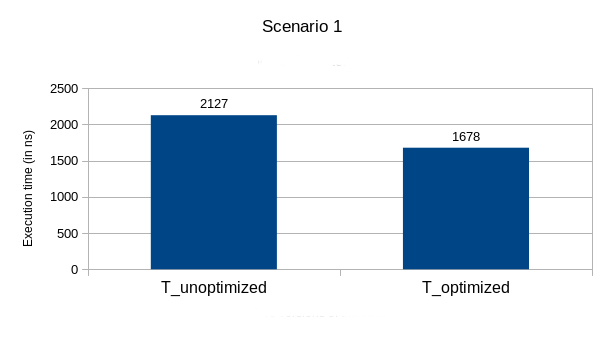
\includegraphics[scale=0.9]{scenario_1.png}
	\caption{Execution times for Scenario 1}
	\label{TC_1}	
\end{figure}

\subsubsection{Scenario 2}

The optimization quality is proportional to the number of array accesses in the loop. This is depicted by this scenario which involves only one array access. 

The results of applying our optimization are

\begin{figure}[H]
	\centering
	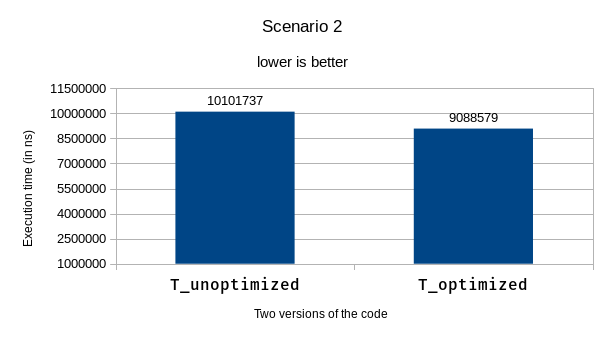
\includegraphics[scale=0.9]{scenario_2.png}
	\caption{Execution times for Scenario 2}
	\label{TC_2}	
\end{figure}

\subsubsection{Scenario 3}

Not applying the optimization when not needed is also an evaluation of our system. Therefore, this scenario contains code which cannot be optimized.

The results of applying our optimization are depicted in \ref{TC_3}

\begin{figure}[H]
	\centering
	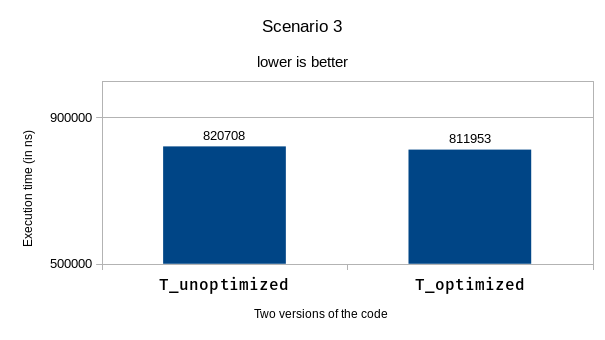
\includegraphics[scale=0.9]{scenario_3.png}
	\caption{Execution times for Scenario 3}
	\label{TC_3}	
\end{figure}

%\pagebreak

\subsection{Evaluation}

For each test case, we then find the RIP according to our formula. The results are below 

\begin{figure}[H]
	\centering
	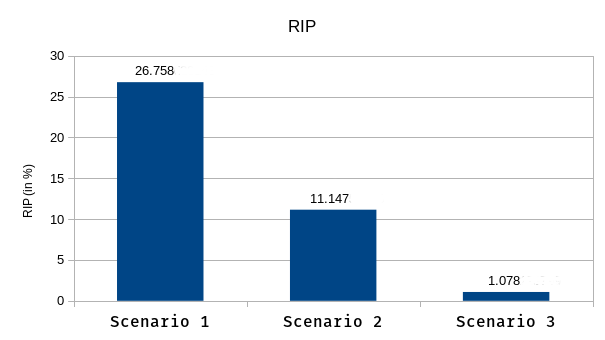
\includegraphics[scale=0.9]{rip_new.png}
	\caption{RIP of all scenarios}
	\label{RIP}	
\end{figure}

\pagebreak

We can deduce the following observations

\begin{enumerate}
	\item The performance is directly proportional to the number of array accesses present in the loop.
	\item There is no improvement or deterioration when the optimized is not applicable. 
\end{enumerate}
 % Testing
% Chapter 6
 % Results
% Chapter 7

\chapter{CONCLUSION AND FUTURE WORK} % Write in your own chapter title
\section{Contribution}

Array access is the costliest memory operation in a standard program, since other accesses do not involve any calculation before accessing the memory location itself. This project implements second order predictive commoning in LLVM compiler infrastructre as a loadable module. The loadablity ensures that it does not necessitate that entire LLVM infrastructure be compiled with this module to make use of this optimization. With appropriate version of Clang, we can dynamically load this module with any version of LLVM later than 3.
\section{Future work}
The loadable module is invoked using a special flag when invoking the compiler. Second order predictive commoning can help drastically reduce the number of loads and stores, which are among the costliest memory operations. Array accesses are dominant in many calculations, including common operations like JPEG and MPEG decoding. All programs that have need for significant repetitive array accesses, may be compiled with this improvement in clang and LLVM, to take advantage of this fact. As an improvement over this project, we can eliminate the need to have a specific form of array access to be optimized, and generalize it to cover even more array access formats. 

We can also send the patch to upstream developers, and merge it to the mainline release in the next LLVM release schedule. This will enable us to get a closer code scrutiny, and will help us in identifying ways to further generalize this optimization, with the help of more experienced LLVM maintainers.  % Conclusion
%
\appendix
% Appendix A

\chapter{Secure Shell (SSH)}
SSH uses public-key cryptography to authenticate the remote computer and allow it to authenticate the user, if necessary. There are several ways to use SSH; one is to use automatically generated public-private key pairs to simply encrypt a network connection, and then use password authentication to log on.

Another is to use a manually generated public-private key pair to perform the authentication, allowing users or programs to log in without having to specify a password. In this scenario, anyone can produce a matching pair of different keys (public and private). The public key is placed on all computers that must allow access to the owner of the matching private key (the owner keeps the private key secret). While authentication is based on the private key, the key itself is never transferred through the network during authentication. SSH only verifies whether the same person offering the public key also owns the matching private key. In all versions of SSH it is important to verify unknown public keys, i.e. associate the public keys with identities, before accepting them as valid. Accepting an attacker's public key without validation will authorize an unauthorized attacker as a valid user.
\section{ Sample Working Code for SSH}
   
\begin{lstlisting}

using System;
using System.Collections.Generic;
using System.Linq;
using System.Text;
using System.Windows;
using System.Windows.Controls;
using System.Windows.Data;
using System.Windows.Documents;
using System.Windows.Input;
using System.Windows.Media;
using System.Windows.Media.Imaging;
using System.Windows.Navigation;
using System.Windows.Shapes;
using Renci.SshNet;

namespace Kinect.Toolbox
{
    public static class ssh
    {
        public static void right()
        {

            {
                try
                {
                    using (var client = new SshClient("192.168.0.104", "pi", "teddy"))
                    {
                        client.Connect();
                        client.RunCommand("sudo python robotright.py");
                        client.Disconnect();
                    }


                }
                catch
                {

                }
            }
        }
        public static void left()
        {

            {
                try
                {
                    using (var client = new SshClient("192.168.0.104", "pi", "teddy"))
                    {
                        client.Connect();
                        client.RunCommand("sudo python robotleft.py");
                        client.Disconnect();
                    }


                }
                catch
                {

                }
            }
        }
        public static void circle()
        {

            {
                try
                {
                    using (var client = new SshClient("192.168.0.104", "pi", "teddy"))
                    {
                        client.Connect();
                        client.RunCommand("sudo python robotcircle.py");
                        client.Disconnect();
                    }


                }
                catch
                {

                }
            }
        }
        public static void up()
        {

            {
                try
                {
                    using (var client = new SshClient("192.168.0.104", "pi", "teddy"))
                    {
                        client.Connect();
                        client.RunCommand("sudo python robotup.py");
                        client.Disconnect();
                    }


                }
                catch
                {

                }
            }
        }
        public static void down()
        {

            {
                try
                {
                    using (var client = new SshClient("192.168.0.104", "pi", "teddy"))
                    {
                        client.Connect();
                        client.RunCommand("sudo python robotdown.py");
                        client.Disconnect();
                    }


                }
                catch
                {

                }
            }
        }
    }
}
\end{lstlisting}
    
\subsection{Sample Swipe Code}
\begin{lstlisting}
using System;
using Microsoft.Kinect;

namespace Kinect.Toolbox
{
    public class SwipeGestureDetector : GestureDetector
    {
        public float SwipeMinimalLength {get;set;}
        public float SwipeMaximalHeight {get;set;}
        public int SwipeMininalDuration {get;set;}
        public int SwipeMaximalDuration {get;set;}

        public SwipeGestureDetector(int windowSize = 20)
            : base(windowSize)
        {
            SwipeMinimalLength = 0.4f;
            SwipeMaximalHeight = 0.2f;
            SwipeMininalDuration = 250;
            SwipeMaximalDuration = 1500;
        }

        protected bool ScanPositions(Func<Vector3, Vector3, bool> heightFunction, Func<Vector3, Vector3, bool> directionFunction, 
            Func<Vector3, Vector3, bool> lengthFunction, int minTime, int maxTime)
        {
            int start = 0;

            for (int index = 1; index < Entries.Count - 1; index++)
            {
                if (!heightFunction(Entries[0].Position, Entries[index].Position) || !directionFunction(Entries[index].Position, Entries[index + 1].Position))
                {
                    start = index;
                }

                if (lengthFunction(Entries[index].Position, Entries[start].Position))
                {
                    double totalMilliseconds = (Entries[index].Time - Entries[start].Time).TotalMilliseconds;
                    if (totalMilliseconds >= minTime && totalMilliseconds <= maxTime)
                    {
                        return true;
                    }
                }
            }

            return false;
        }

        protected override void LookForGesture()
        {
            // Swipe to right
            if (ScanPositions((p1, p2) => Math.Abs(p2.Y - p1.Y) < SwipeMaximalHeight, // Height
                (p1, p2) => p2.X - p1.X > -0.01f, // Progression to right
                (p1, p2) => Math.Abs(p2.X - p1.X) > SwipeMinimalLength, // Length
                SwipeMininalDuration, SwipeMaximalDuration)) // Duration
            {
               RaiseGestureDetected("SwipeToRight");
               ssh.right();
                return;
            }

            // Swipe to left
            if (ScanPositions((p1, p2) => Math.Abs(p2.Y - p1.Y) < SwipeMaximalHeight,  // Height
                (p1, p2) => p2.X - p1.X < 0.01f, // Progression to right
                (p1, p2) => Math.Abs(p2.X - p1.X) > SwipeMinimalLength, // Length
                SwipeMininalDuration, SwipeMaximalDuration))// Duration
            {
               RaiseGestureDetected("SwipeToLeft");
               ssh.left();
                return;
            }
            if (ScanPositions((p1, p2) => Math.Abs(p2.X - p1.X) < SwipeMaximalHeight, // Height
                (p1, p2) => p2.Y - p1.Y > -0.01f, // Progression to up
                (p1, p2) => Math.Abs(p2.Y - p1.Y) > SwipeMinimalLength, // Length
                SwipeMininalDuration, SwipeMaximalDuration)) // Duration
            {
                RaiseGestureDetected("SwipetoUp");
                ssh.up();
                return;
            }
            if (ScanPositions((p1, p2) => Math.Abs(p2.X - p1.X) < SwipeMaximalHeight,  // Height
                (p1, p2) => p2.Y - p1.Y < 0.01f, // Progression to down
                (p1, p2) => Math.Abs(p2.Y - p1.Y) > SwipeMinimalLength, // Length
                SwipeMininalDuration, SwipeMaximalDuration))// Duration
            {
                RaiseGestureDetected("SwipeToDown");
                ssh.down();
                return;
            }
        }
    }
}
\end{lstlisting}       
\section{Sample Circle Code}
\begin{lstlisting}
using System.Linq;
using System.IO;
using Microsoft.Kinect;

namespace Kinect.Toolbox
{
    public class TemplatedGestureDetector : GestureDetector
    {
        public float Epsilon { get; set; }
        public float MinimalScore { get; set; }
        public float MinimalSize { get; set; }
        readonly LearningMachine learningMachine;
        RecordedPath path;
        readonly string gestureName;

        public bool IsRecordingPath
        {
            get { return path != null; }
        }

        public LearningMachine LearningMachine
        {
            get { return learningMachine; }
        }

        public TemplatedGestureDetector(string gestureName, Stream kbStream, int windowSize = 60)
            : base(windowSize)
        {
            Epsilon = 0.035f;
            MinimalScore = 0.80f;
            MinimalSize = 0.1f;
            this.gestureName = gestureName;
            learningMachine = new LearningMachine(kbStream);
        }

        public override void Add(SkeletonPoint position, KinectSensor sensor)
        {
            base.Add(position, sensor);

            if (path != null)
            {
                path.Points.Add(position.ToVector2());
            }
        }

        protected override void LookForGesture()
        {
            if (LearningMachine.Match(Entries.Select(e => new Vector2(e.Position.X, e.Position.Y)).ToList(), Epsilon, MinimalScore, MinimalSize))
            {
                RaiseGestureDetected(gestureName);
                ssh.circle();
            }
        }

        public void StartRecordTemplate()
        {
            path = new RecordedPath(WindowSize);
        }

        public void EndRecordTemplate()
        {
            LearningMachine.AddPath(path);
            path = null;
        }

        public void SaveState(Stream kbStream)
        {
            LearningMachine.Persist(kbStream);
        }
    }
}
\end{lstlisting}	% 
%
\backmatter
\bibliographystyle{aubecse}
\bibliography{bethesis}

\end{document}
